\chapter{Background \& Objectives}

% This section should discuss your preparation for the project, including background
% reading, your analysis of the problem and the process or method you have followed
% to help structure your work.  It is likely that you will reuse part of your outline
% project specification, but at this point in the project you should have more to talk about.

\section{Background}
% What was your background preparation for the project? What similar systems did
% you assess? What was your motivation and interest in this project?

\subsection{Motivation}
I enjoy programming, and this project seemed to involve a lot of coding. I was also excited
to build a complex, real time system, while applying my previous software engineering
experience and learning new technologies at the same time. I knew I would be given
a lot of freedom to choose the most appropriate tools for the task, and incorporate
modern software development practices, including continuous integration and
containerised environments, to deliver good quality software. I was also keen on developing something that could be actually
useful to the university once I leave Aberystwyth. It is more motivating to develop
a product, while knowing it could be potentially used in real life, as opposed to being
forgotten after the submission. I have experienced being presented with wrong slides
during a lecture in my first year at university, so I was happy to address the problem
of a single session Qwizdom license with my tool.

\subsection{Technology Considerations}
\subsubsection{Programming Languages}
% - Initial proposal to create an Android based system for students -> React Native -> MEAN
The initial proposal was to create the classroom quiz system using Java\cite{3} to run it natively
on Android\cite{4} mobile devices. The lecturer was supposed the create quizzes on his teaching
machine, by interacting with the system using a web front end. Lecture slides were then supposed
to be broadcasted to his audience, and they could use their mobile phones to answers questions,
which would be then sent back to the lecturer for analysis. I have had previous experience with
native Android development, therefore this approach seemed like a reasonable option. The only problem was,
iOS\cite{5} devices are very popular in the United Kingdom, and developing an app for Android would exclude
a good percentage of students from being able to actively participate in lectures presented. I have
therefore started to think about alternative approaches.

The second possibility was to use React Native\cite{6}, a JavaScript\cite{7} framework allowing
developers to create mobile applications in JavaScript and compile it down to both iOS and Android.
This approach would still require the web front end for the lecturer to be developed, and a natural
choice would be to use React\cite{8} to keep the learning curve as low as possible.

The final alternative considered, was to develop the whole tool as a web application. This way both the
front end for lecturers and students could be developed using the same framework. Members of the audience
could participate in lectures by accessing the web application using web browsers installed
both on their mobile phones, regardless of the operating system, and their laptops. I considered
both React and Angular 4\cite{9}, since I have already briefly used it before. React is a library
for developing user interface, whereas Angular is a web development framework. The only caveat with
using Angular is that the developer needs to learn TypeScript\cite{10}, which compiles down to JavaScript.

\subsubsection{The WebSocket Protocol}
The Quiz Tool was supposed to allow a lecturer to broadcast his slides to all the students
participating in a lecture. This requires a bidirectional communication protocol between the
server and the clients. For example, if a lecturer emits the next slide of his presentation,
this change should be pushed to the back end, and then the back end needs to be able to
send the new slide to all the students. Students' clients should also be able to push quiz
answers back to the back end, so they can be presented to the lecturer in some form.

The WebSocket Protocol can be used to create such real time systems. It enables two-way
communication between a client and a remote host, making it ideal for instant messaging,
gaming applications, and the Quiz Tool. It uses a single TCP connection for trafic
in both directions\cite{11}.

\subsubsection{Prototyping}
I have followed various tutorials to quickly prototype proof of concept applications,
in order to learn more about the technologies which could be useful during the Quiz Tool
development. I started with the Socket.io chat tutorial. Socket.io is
a JavaScript library enabling bidirectional event-based communication, and uses
the WebSocket Protocol internally\cite{12}. I have created a chat application following one
of the tutorials on their homepage\cite{13}. I have also learned the basics of
Angular by following the Tour of Heroes tutorial\cite{14}, and finally tried to
understand how Angular could work together with Socket.io by following the MEAN
Socket.io tutorial\cite{15}.

\subsection{On-site vs External Hosting}
% - local LSX container vs external cloud provider -> LDAP
The initial plan to handle authentication in Quiz Tool was to use the university
LDAP\cite{16}. This way, lecturers would be able to provide their university credentials,
which would be checked using the Bind operation against the university directory of users,
to check if a given person is authorised to use the tool. This would require the Quiz Tool
to be deployed to a production environment running within the university intranet. The
alternative was to deploy the application to an external cloud hosting.

\subsection{Similar Tools}
Qwizdom\cite{1}, is the tool currently used by the university to embed quizzes into
presentations to judge students' understanding of the content presented. It has to be
installed on lecturer's machine as it is a desktop application. Qwizdom integrates
with Microsoft PowerPoint\cite{17}, by adding an extra toolbar allowing the lecturer
to insert quiz questions into his presentations and then broadcast them. Once
a presentation is started, a session key appears which can be shared with the audience.
They can then use the key to join the lecture and answer questions once they become available.

\begin{figure}[ht]
    \centering
    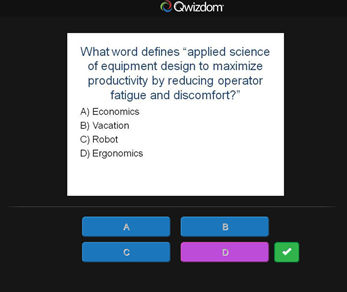
\includegraphics[]{qwizdom.png}
    \caption{Qwizdom web view for the audience}
    \label{fig:qwizdom}
\end{figure}

\section{Analysis}
% Taking into account the problem and what you learned from the background work,
% what was your analysis of the problem? How did your analysis help to decompose
% the problem into the main tasks that you would undertake? Were there alternative
% approaches? Why did you choose one approach compared to the alternatives?
%
% There should be a clear statement of the objectives of the work, which you will
% evaluate at the end of the work.
%
% In most cases, the agreed objectives or requirements will be the result of a compromise
% between what would ideally have been produced and what was determined to be possible in
%  the time available. A discussion of the process of arriving at the final list is usually appropriate.
%
% As mentioned in the lectures, think about possible security issues for the project topic.
%  Whilst these might not be relevant for all projects, do consider if there are relevant
%   for your project. Where there are relevant security issues, discuss how they will
%   this affect the work that you are doing. Carry forward this discussion into relevant
%    areas for design, implementation and testing.

% - MEAN stack \& Docker \& docker-compose
% - Version Control
% - build - Circle CI -> testing, autodeploy
% - AWS Production environment (did not know of Elasticbeanstalk at this point)
% - Google Single Sign On -> Security
% - Identification of major problems
% - Top level requirements of the system
\subsection{MEAN Stack}
Having considered various methods of developing the Quiz Tool, I have decided to
choose the web application approach. Allowing students to access the tool using both
their mobile devices and laptops, combined with the relatively low learning curve
both for me, and for anyone maintaining the software in the future, made it the best
option in my opinion. Furthermore, I have decided to develop the application entirely
in JavaScript based technologies using the MEAN stack\cite{18}.

MEAN stack consists of four elements:
\begin{itemize}
  \item \textbf{M}ongoDB is a JSON document storage NoSQL database
  \item \textbf{E}xpress is a minimalistic JavaScript web development framework
  \item \textbf{A}ngular is a front end web development framework
  \item \textbf{N}odeJS is a JavaScript engine
\end{itemize}

Front ends for both lecturers and students would be written in Angular, NodeJS would be
used on the back end together with Express, and the persistence layer would be provided
by MongoDB.

\subsection{Docker}
Each part of the application would be containerised using Docker\cite{19}, and containers
would run together in the same fashion on the developer's machine, and the build engine
using docker-compose\cite{20} container orchestration tool. Docker is an open source
engine which can be used to wrap an application and all its dependencies into a
lightweight container that can run on any machine capable of running containers\cite{21}.
Docker-compose on the other hand, is a tool for defining and running multi-container
Docker applications.

\subsection{AWS Production Environment}
Unfortunately, the on-site hosting provided by the university to students to deploy
their final projects to was inadequate for the DevOps infrastructure I wanted to
put in place. I wanted to have a machine capable of running docker-compose, and some
form of continuous integration agent. The LXC debian containers\cite{22} were not
compatible with either docker-compose, or Jenkins\cite{23}. The Quiz Tool would be therefore
deployed to the production environment provided by an external cloud provider AWS\cite{24},
and an alternative build agent would be used. The GitHub Student Developer Pack\cite{25} offers
\$150 worth of credits for the Amazon cloud, which is why AWS was chosen.

\subsection{Build}


\subsection{Authentication and Security}

\subsection{Major Problems}

\subsection{Top Level Requirements}

\section{Process}
\subsection{Development Methodology}

\subsection{Version Control}

% You need to describe briefly the life cycle model or research method that you used. You
%  do not need to write about all of the different process models that you are aware of.
%  Focus on the process model that you have used. It is possible that you needed to adapt
%  an existing process model to suit your project; clearly identify what you used and how
%  you adapted it for your needs.
